\begin{problem}[第30届全国中学生物理竞赛复赛][半球面滑块运动]{1}
\begin{wrapfigure}{r}{0.3\textwidth}
    \vspace*{-1.5\baselineskip} 
    \centering
    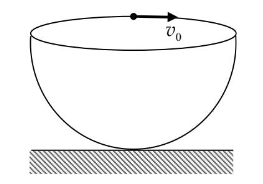
\includegraphics[width=0.9\linewidth]{image/1.png}
\end{wrapfigure}
一半径为 $R$、内侧光滑的半球面固定在地面上，开口水平且朝上。一小滑块在半球面内侧最高点处获得沿球面的水平速度，其大小为 $v_{0}(v_{0} \neq 0)$。求滑块在整个运动过程中可能达到的最大速率。重力加速度大小为 $g$。
\end{problem}
